% =============================================================================
%              CHAPTER 3: MATERIALS AND METHODS
% =============================================================================
\chapter{Materials and Methods}

\section{Overview of Research Methodology}

This research adopts a rigorous, controlled frozen-feature evaluation protocol to compare the representational capabilities of self-supervised video encoders (\vjepaa{}) against instruction-tuned vision-language models (\qwenvl{}). In addition to baseline evaluation, we use a specialized downstream classification architecture HAF-STD Net (Hierarchical Adaptive Fusion with Spectral-Temporal Decomposition) designed to explicitly exploit V-JEPA~2.1's temporal token coherence and hierarchical depth representation space.

The methodology follows a multi-stage experimental pipeline: (1)~Data Acquisition and Sampling, (2)~Spatiotemporal Multi-Layer Feature Extraction, (3)~Feature Preprocessing and Dimensionality Reduction, (4)~Downstream Evaluation across 8 Baseline Classifiers and  HAF-STD Net, and (5)~Comparative Analysis.

Figure~\ref{fig:methodology_pipeline} provides a high-level flowchart depicting the end-to-end experimental architecture.

\begin{figure}[H]
\centering
\begin{tikzpicture}[
    node distance=0.8cm,
    block/.style={rectangle, draw=blue!80!black, fill=blue!5, thick, rounded corners=4pt, text width=4.2cm, text centered, minimum height=1.0cm, font=\normalsize},
    modelblock/.style={rectangle, draw=orange!70!black, fill=orange!8, thick, rounded corners=4pt, text width=4.2cm, text centered, minimum height=1.8cm, font=\normalsize},
    procblock/.style={rectangle, draw=green!60!black, fill=green!5, thick, rounded corners=4pt, text width=10.0cm, text centered, minimum height=1.0cm, font=\normalsize},
    pcablock/.style={rectangle, draw=green!60!black, fill=green!5, thick, rounded corners=4pt, text width=10.0cm, text centered, minimum height=1.0cm, font=\normalsize},
    branchblock/.style={rectangle, draw=green!60!black, fill=green!5, thick, rounded corners=4pt, text width=4.2cm, text centered, minimum height=1.4cm, font=\small},
    trainblock/.style={rectangle, draw=cyan!60!black, fill=cyan!8, thick, rounded corners=4pt, text width=4.2cm, text centered, minimum height=1.4cm, font=\small},
    novelblock/.style={rectangle, draw=red!70!black, fill=red!8, thick, rounded corners=4pt, text width=4.2cm, text centered, minimum height=1.4cm, font=\small},
    resultblock/.style={rectangle, draw=yellow!60!black, fill=yellow!12, thick, rounded corners=4pt, text width=10.0cm, text centered, minimum height=1.0cm, font=\normalsize},
    arrow/.style={->, >=stealth, line width=1.1pt, color=blue!80!black},
    redarrow/.style={->, >=stealth, thick, line width=1.2pt, dashed, red!70!black},
]
    % === Stage 1: Data Sources ===
    \node[block] (fg_src) {\textbf{FineGym}\\1,200 clips\\4 event classes};
    \node[block, right=1.2cm of fg_src] (hmdb_src) {\textbf{HMDB51}\\6,754 clips\\51 action classes};

    % === Stage 2: Frame Extraction ===
    \node[procblock, below=1.0cm of $(fg_src.south)!0.5!(hmdb_src.south)$] (frames) {\textbf{Frame Extraction \& Normalization}\\OpenCV \texttt{VideoCapture} $\rightarrow$ Uniform temporal sampling $\rightarrow$ Resize to $224\times224$};

    % === Stage 3: Feature Extractors ===
    \node[modelblock, below left=1.2cm and 0.8cm of frames.south] (vjepa) {\textbf{V-JEPA~2.1 (654M)}\\ViT-Huge (float16)\\8 frames $\rightarrow$ 4 layers\\$\times\;T'\!\times\!1280$};
    \node[modelblock, below right=1.2cm and 0.8cm of frames.south] (qwen) {\textbf{Qwen2.5-VL (7B)}\\4-bit NF4 quantized\\4 frames $\rightarrow$ 3584-d\\hidden-state pooling};

    % === Stage 4a: Feature Preprocessing — StandardScaler (all classifiers) ===
    \node[procblock, below=1.2cm of $(vjepa.south)!0.5!(qwen.south)$] (scaler) {\textbf{Feature Preprocessing}\\StandardScaler (zero mean, unit variance) $\rightarrow$ 80/20 Train/Eval Split};

    % === Stage 4b: PCA Dimensionality Reduction (baseline classifiers only) ===
    \node[pcablock, below=0.9cm of scaler] (pca) {\textbf{PCA Dimensionality Reduction}\\95\% variance retained $\rightarrow$ compact subspace ($k^* \ll D$)};

    % === Stage 5: Classifier Branches ===
    % HAF-STD Net (far left — multi-layer features, uses StandardScaler but bypasses PCA)
    \node[novelblock, below left=1.4cm and 3.5cm of pca.south] (hafstd) {\textbf{HAF-STD Net}\\{\scriptsize 4.8M params}};
    % Classical ML (center — shared path, both models)
    \node[branchblock, below=1.4cm of pca] (classify_sk) {\textbf{Classical ML (3)}\\SVM-RBF $\cdot$ Random Forest\\LogReg};
    % Neural Network Classifiers (right — shared path, both models)
    \node[trainblock, below right=1.4cm and 3.5cm of pca.south] (classify_pt) {\textbf{Neural Network Classifiers (5)}\\MLP $\cdot$ DeepMLP $\cdot$ ResMLP\\Conv1DNet $\cdot$ Transformer\\{\scriptsize LS + Mixup + CosLR}};

    % === Stage 6: Comparative Evaluation ===
    \node[resultblock, below=1.4cm of classify_sk] (results) {\textbf{Comparative Evaluation and Analysis}\\Top-1 Acc, Macro/Weighted F1, MCC, Cohen's $\kappa$, Top-5 Accuracy};

    % ====== ARROWS ======

    % Data sources -> Frame extraction
    \draw[arrow] (fg_src.south) -- (fg_src.south |- frames.north);
    \draw[arrow] (hmdb_src.south) -- (hmdb_src.south |- frames.north);

    % Frame extraction -> Models
    \draw[arrow] (frames.south -| vjepa.north) -- (vjepa.north);
    \draw[arrow] (frames.south -| qwen.north) -- (qwen.north);

    % Models -> StandardScaler (mean-pooled features for baselines)
    \draw[arrow] (vjepa.south) -- (vjepa.south |- scaler.north)
        node[midway, right, font=\scriptsize\itshape, text=black!60] {Mean-pooled};
    \draw[arrow] (qwen.south) -- (qwen.south |- scaler.north);

    % V-JEPA multi-layer features -> StandardScaler (HAF-STD path enters preprocessing)
    \draw[redarrow] (vjepa.west) -- node[above, font=\scriptsize\itshape, text=red!70!black, align=center] {Multi-layer\\features} ++(-1.2, 0) |- (scaler.west);

    % StandardScaler -> PCA (baseline path)
    \draw[arrow] (scaler.south) -- (pca.north);

    % StandardScaler -> HAF-STD Net (bypasses PCA)
    \draw[redarrow] (scaler.south west) ++(0.3,0) -- ++(0,-.45) -| (hafstd.north);

    % PCA -> Shared classifier branches (two-way fan)
    \coordinate (fan) at ($(pca.south) + (0,-0.8)$);
    \draw[thick, color=blue!80!black] (pca.south) -- (fan);
    \draw[arrow] (fan) -- (classify_sk.north);
    \draw[arrow] (fan) -| (classify_pt.north);

    % Shared classifiers -> Comparative Evaluation (fan-in)
    \coordinate (merge) at ($(classify_sk.south) + (0,-0.8)$);
    \draw[thick, color=blue!80!black] (classify_sk.south) -- (merge);
    \draw[arrow] (merge) -- (results.north);
    \draw[arrow] (classify_pt.south) |- (merge);

    % HAF-STD -> Comparative Evaluation (dashed red path along left side)
    \draw[redarrow] (hafstd.south) |- (results.west);

\end{tikzpicture}

\caption{Flowchart depicting the proposed multi-stage experimental methodology pipeline. Solid arrows indicate the shared baseline path where mean-pooled features from both models undergo StandardScaler normalization and PCA dimensionality reduction before evaluation by 8 baseline classifiers. Dashed red arrows indicate the HAF-STD Net path, which routes V-JEPA~2.1's multi-layer temporal features through StandardScaler normalization but bypasses PCA.}
\label{fig:methodology_pipeline}
\end{figure}


\section{Data Acquisition and Dataset Characteristics}


To evaluate model performance across different task granularities, two benchmark datasets of contrasting complexity are utilized:

\subsection{FineGym Dataset (Fine-Grained Action Recognition)}
FineGym is a fine-grained activity recognition benchmark containing high-frame-rate competitive gymnastics footage. The official annotation file (v1.1) specifies precise temporal boundaries and hierarchical activity labels. In this study, evaluation focuses on the top-level Event classification tier, comprising 4 distinct gymnastics apparatus events: Balance Beam (BB), Floor Exercise (FX), Uneven Bars (UB), and Vault (VT). A balanced sample of 300 clips per class (1,200 total clips) is targeted for download via \texttt{yt-dlp} from YouTube.

\subsection{HMDB51 Dataset (General Action Recognition)}
HMDB51 is a classic benchmark for general human action recognition, curated from commercial movies and web videos. It comprises 6,754 video clips categorized into 51 action classes, encompassing facial expressions, general body motion, human-object interactions, and human-human interactions. The complete dataset is ingested directly from the Hugging Face Hub repository (\texttt{jili5044/hmdb51}).

Table~\ref{tab:dataset_comparison} summarizes the structural properties and comparative parameters of both benchmark datasets.

\begin{table}[H]
\centering
\caption{Comparison of FineGym and HMDB51 benchmark dataset specifications.}
\label{tab:dataset_comparison}
\begin{tabular}{lrr}
\toprule
\textbf{Dataset Parameter} & \textbf{FineGym (Event Level)} & \textbf{HMDB51} \\
\midrule
Task Granularity & Fine-grained (Gymnastics) & Coarse-grained (General) \\
Number of Classes & 4 & 51 \\
Target Sample Size & 1,200 clips & 6,754 clips \\
Domain Context & Uniform arena/gym environment & Diverse real-world settings \\
Primary Discriminative Cue & Subtle body kinematics & Broad motion \& background \\
Evaluation Split & 80\% Train / 20\% Test & 80\% Train / 20\% Test \\
\bottomrule
\end{tabular}
\end{table}

\section{Data Preprocessing and Input Pipeline}

Video clips undergo standardized preprocessing prior to feature extraction:
\begin{enumerate}[leftmargin=*]
    \item \textbf{Uniform Temporal Frame Sampling:} For a video clip containing $N$ total frames, a sequence of $N_f$ frames is uniformly sampled along the temporal axis:
    \begin{equation*}
        t_i = \left\lfloor i \cdot \frac{N}{N_f} \right\rfloor, \quad i \in \{0, 1, \dots, N_f - 1\}
    \end{equation*}
    For \vjepaa{}, $N_f = 8$ frames are sampled; for \qwenvl{}, $N_f = 4$ frames are sampled.
    \item \textbf{Spatial Resizing and Normalization:} Sampled frames are resized to $224 \times 224$ pixels and normalized using standard ImageNet mean ($\boldsymbol{\mu} = [0.485, 0.456, 0.406]$) and standard deviation ($\boldsymbol{\sigma} = [0.229, 0.224, 0.225]$).
\end{enumerate}

\section{Feature Extraction Framework}

Both candidate models function strictly as frozen feature extractors without updating backbone parameters.

\subsection{Self-Supervised Encoder: \vjepaa{}}
\vjepaa{} \citep{assran2025vjepa2} utilizes a ViT-Huge backbone (654M parameters) trained via non-generative spatiotemporal prediction in a latent embedding space. Given an input video sequence of 8 sampled frames, we extract two feature representations:
\begin{enumerate}[leftmargin=*]
    \item \textbf{Multi-Layer Per-Frame Features (for HAF-STD Net):} Hidden states are extracted from 4 intermediate encoder layers at 25\%, 50\%, 75\%, and 100\% depth. Spatial tokens are mean-pooled per frame, producing a tensor $\mathbf{H}_{\text{multi}} \in \mathbb{R}^{4 \times T' \times 1280}$ per clip that preserves both depth hierarchy and temporal structure.
    \item \textbf{Global Mean-Pooled Features (for Baseline Probes):} Global average pooling across all spatiotemporal tokens of the final layer outputs $\mathbf{f}_{\text{VJEPA}} \in \mathbb{R}^{1280}$.
\end{enumerate}

\subsection{V-JEPA~2.1 Self-Supervised Training Objectives}

The representational quality of the frozen \vjepaa{} encoder stems from its self-supervised pretraining objective, which performs \emph{mask-denoising prediction in representation space} rather than pixel reconstruction. Given two views $x$ and $y$ of a video, where patches have been randomly dropped from $y$, the encoder $E_\theta(\cdot)$ extracts representations from the unmasked view $x$, and a predictor $P_\phi(\cdot)$ predicts the representation of the masked view. The training objective minimizes the $\ell_1$ distance between predicted and target representations \citep{assran2025vjepa2}:
\begin{equation*}
    \underset{\theta,\,\phi,\,\Delta_y}{\text{minimize}} \quad \|P_\phi(\Delta_y, E_\theta(x)) - \operatorname{sg}(E_{\bar{\theta}}(y))\|_1
\end{equation*}
where $\Delta_y$ is a learnable mask token that indicates the locations of the dropped patches, $\operatorname{sg}(\cdot)$ denotes a stop-gradient operator to prevent representation collapse, and $\bar{\theta}$ represents an exponential moving average (EMA) of the encoder weights $\theta$. The loss is applied only to predictions of masked patches, and both the encoder $E_\theta(\cdot)$ and predictor $P_\phi(\cdot)$ are parameterized as Vision Transformers (ViTs) with Rotary Position Embedding (RoPE).

V-JEPA~2.1 \citep{murlabadia2026vjepa21} refines this objective by introducing a \emph{dense per-token prediction loss} that applies supervision individually to each masked spatiotemporal token rather than globally:
\begin{equation*}
    \mathcal{L}_{\text{predict}} = \frac{1}{|M|} \sum_{i \in M} \|P_\phi(E_\theta(x), \Delta_y)_i - \operatorname{sg}(E_{\bar{\theta}}(y)_i)\|_1
\end{equation*}
where $M$ is the set of masked patch indices from the $x$ view, and the subscript $i$ denotes the $i$-th token position. This dense formulation, combined with multi-layer intermediate supervision across encoder depth, enhances the spatial and temporal grounding of learned representations.

Figure~\ref{fig:vjepa2_arch} illustrates the complete V-JEPA~2.1 pretraining architecture. The dual-encoder framework consists of an x-Encoder $E_\theta$ that processes unmasked context tokens and a y-Encoder $E_{\bar{\theta}}$ (updated via EMA) that produces target representations. A multi-level predictor $P_\phi$ reconstructs the masked spatiotemporal token representations by fusing features across multiple encoder depths, with two complementary loss terms: a context loss ($\lambda_d \cdot L_1$) and a prediction loss ($L_1$), both applied through stop-gradient operations to prevent representational collapse.

\begin{figure}[H]
\centering
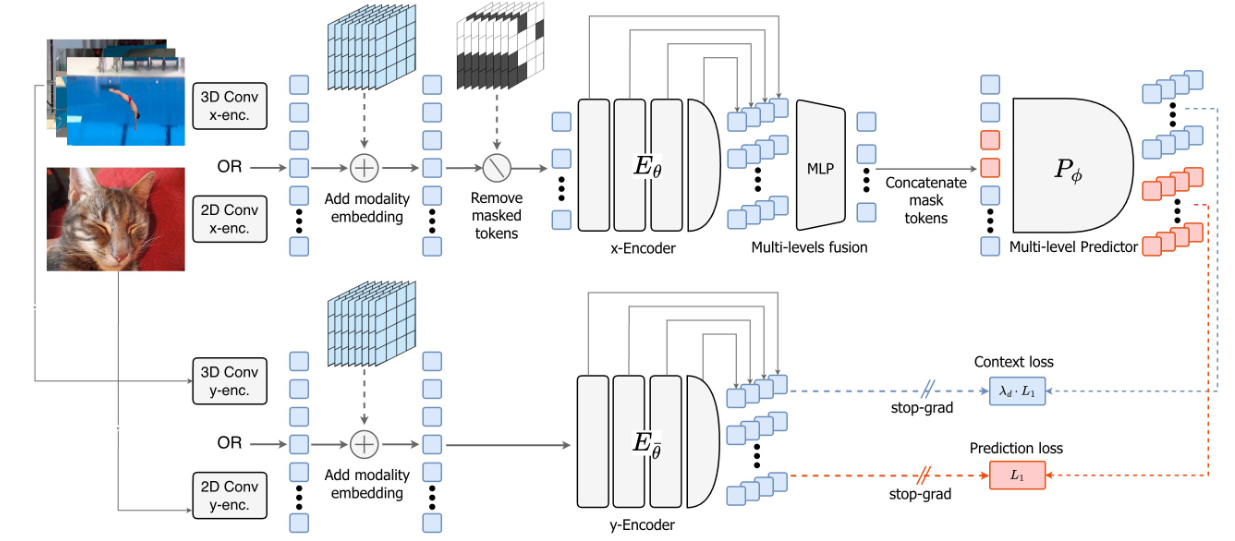
\includegraphics[width=\textwidth]{../fig/vjepa2.png}
\caption{Architecture of V-JEPA~2.1 self-supervised pretraining framework showing the dual x-Encoder and y-Encoder pipeline with multi-level fusion, mask-denoising prediction, and stop-gradient targets \citep{murlabadia2026vjepa21}.}
\label{fig:vjepa2_arch}
\end{figure}

\subsection{Vision-Language Model: \qwenvl{}}
\qwenvl{} \citep{qwen2025qwen3vl} (7B parameters) integrates a Vision Transformer encoder with a language model decoder. The model is loaded in 4-bit NormalFloat (NF4) quantization \citep{pathak2026efficientvlms}. The 4 sampled frames are passed alongside a minimal prompt (\texttt{"Describe the video action."}). The output hidden state of the final decoder layer $\mathbf{H}_{\text{decoder}} \in \mathbb{R}^{S \times 3584}$ is average-pooled across sequence tokens:
\begin{equation*}
    \mathbf{f}_{\text{Qwen}} = \frac{1}{S} \sum_{s=1}^{S} \mathbf{h}_s \in \mathbb{R}^{3584}
\end{equation*}

Figure~\ref{fig:qwen_arch} depicts the Qwen2.5-VL architecture. The model employs a Vision Encoder with a Conv3D patch embedding layer and window-partitioned attention blocks, which processes images and video frames at their native resolution. Visual tokens are then projected and interleaved with text tokens into the Qwen2.5 Language Model (LM) Decoder for autoregressive generation. Notably, the architecture uses Multimodal Rotary Position Embedding (MRoPE) with absolute time alignment for temporal grounding of video inputs and dynamic FPS sampling to accommodate variable-length video sequences.

\begin{figure}[H]
\centering
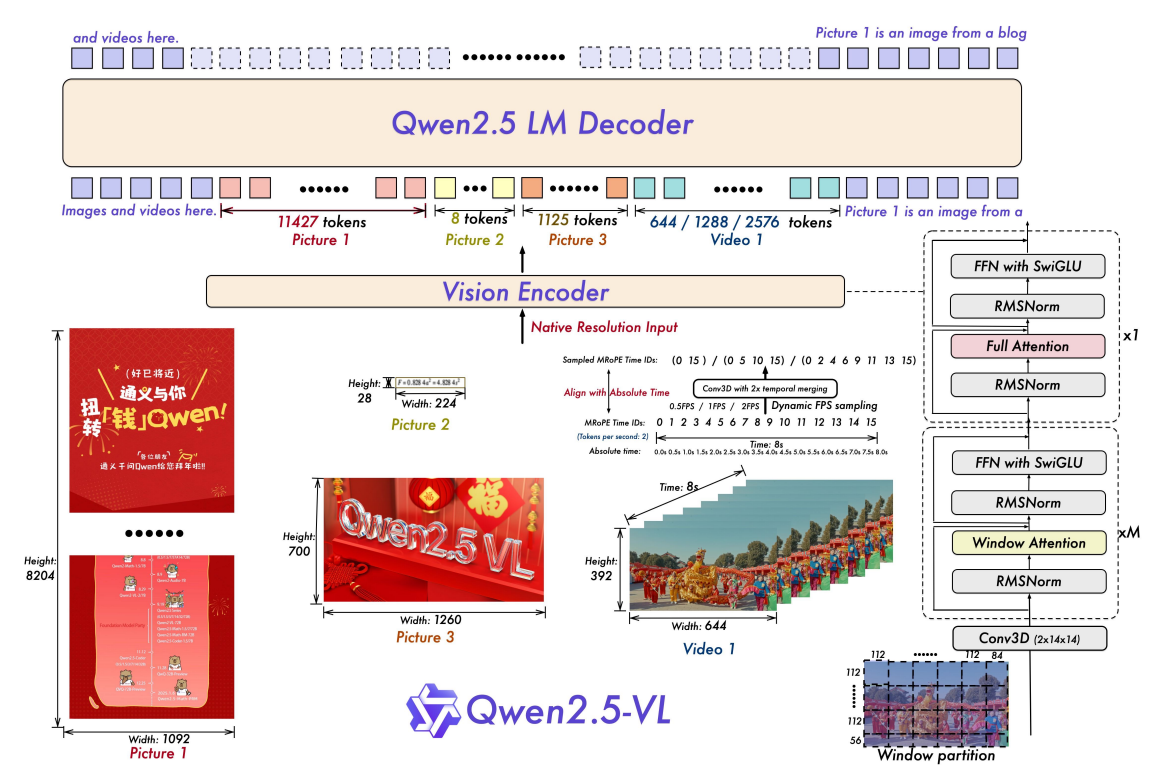
\includegraphics[width=\textwidth]{../fig/qwen.png}
\caption{Architecture of Qwen2.5-VL vision-language model illustrating the Vision Encoder with Conv3D patch embedding, window attention, and native resolution input processing, feeding into the Qwen2.5 LM Decoder with MRoPE temporal alignment \citep{qwen2025qwen3vl}.}
\label{fig:qwen_arch}
\end{figure}

\section{Feature Standardization and Dimensionality Reduction}

To ensure optimal classifier convergence and mitigate the curse of dimensionality, extracted feature vectors undergo standard transformations:
\begin{enumerate}[leftmargin=*]
    \item \textbf{Z-Score Standardization:} Feature vectors $\mathbf{x}_i$ are standardized using training set statistics:
    \begin{equation*}
        \mathbf{z}_i = \frac{\mathbf{x}_i - \boldsymbol{\mu}_{\text{train}}}{\boldsymbol{\sigma}_{\text{train}}}
    \end{equation*}
    \item \textbf{Principal Component Analysis (PCA):} PCA is fitted on the standardized training feature matrix $\mathbf{Z}_{\text{train}}$ to project representations onto an orthogonal subspace while retaining 95\% of total variance:
    \begin{equation*}
        K = \arg\min_k \left\{ \frac{\sum_{j=1}^k \lambda_j}{\sum_{m=1}^D \lambda_m} \ge 0.95 \right\}
    \end{equation*}
\end{enumerate}

\section{Downstream Baseline Classifiers}

An ensemble of 8 baseline classifiers (3 classical ML and 5 neural network classifiers) is evaluated on the transformed feature representations:

\subsection{Classical Machine Learning Classifiers}
\begin{enumerate}[leftmargin=*]
    \item \textbf{Support Vector Machine (SVM-RBF):} RBF kernel with $C=10.0$ and balanced class weighting.
    \item \textbf{Random Forest:} Ensemble of 500 decision trees with Gini impurity split criteria.
    \item \textbf{Softmax Logistic Regression:} Multinomial linear probe with L2 regularization ($C=1.0$).
\end{enumerate}

\subsection{Neural Network Classifier Architectures}
\begin{enumerate}[leftmargin=*]
    \item \textbf{Multi-Layer Perceptron (MLP):} Scikit-learn MLP with two hidden layers (512, 256) and adaptive learning rate.
    \item \textbf{DeepMLP:} 4-layer feedforward network (512 $\rightarrow$ 256 $\rightarrow$ 128 $\rightarrow$ Classes) with BatchNorm, GELU, and Dropout (0.3).
    \item \textbf{ResMLP:} Deep residual MLP with 3 residual blocks: $\mathbf{h}_{l+1} = \text{GELU}(\mathbf{h}_l + \mathcal{F}(\mathbf{h}_l))$.
    \item \textbf{Conv1DNet:} 1D CNN treating feature dimensions as sequence channels.
    \item \textbf{MiniTransformer:} 2-layer Transformer Encoder with multi-head self-attention ($h=4$) on chunked feature embeddings.
\end{enumerate}

All neural network baseline models are trained using label smoothing ($\epsilon=0.1$), feature-space mixup ($\alpha=0.2$), Cosine Annealing LR scheduling, and early stopping.

\section{Proposed Classifier Architecture: HAF-STD Net}
\label{sec:proposal_hafstd}

As a key technical contribution of this thesis, we propose HAF-STD Net (Hierarchical Adaptive Fusion with Spectral-Temporal Decomposition), a classification architecture (4.8M parameters) specifically tailored for frozen V-JEPA~2.1 backbones. HAF-STD Net operates on multi-layer per-frame features $\mathbf{H} \in \mathbb{R}^{4 \times T' \times 1280}$ and incorporates three core mechanisms:

\subsection{1. Spectral-Temporal Decomposition via 1D Haar DWT}
At each selected layer $k \in \{1, 2, 3, 4\}$, a 1D Haar Discrete Wavelet Transform is applied along the temporal dimension $T'$:
\begin{equation*}
    \mathbf{a}_k = \frac{1}{2}(\mathbf{h}_{2t} + \mathbf{h}_{2t+1}), \quad
    \mathbf{d}_k = \frac{1}{2}(\mathbf{h}_{2t} - \mathbf{h}_{2t+1})
\end{equation*}
where $\mathbf{a}_k$ isolates low-frequency static appearance features and $\mathbf{d}_k$ isolates high-frequency motion dynamics.

\subsection{2. Inter-Layer Representation Velocity}
Inter-layer deltas are computed between consecutive encoder layers to quantify representation velocity across depth:
\begin{equation*}
    \Delta\mathbf{H}_k = \bar{\mathbf{H}}_{k+1} - \bar{\mathbf{H}}_k
\end{equation*}
where $\bar{\mathbf{H}}_k$ is the temporally mean-pooled representation at layer $k$.

\subsection{3. Adaptive Routing and Cosine Classification}
The 3 streams per layer (appearance, motion, velocity) yield $4 \times 3 = 12$ projected feature streams $\mathbf{s}_i \in \mathbb{R}^{256}$. An adaptive routing network computes input-dependent softmax weights $\mathbf{w} \in \mathbb{R}^{12}$:
\begin{equation*}
    \mathbf{w} = \text{softmax}\left(\text{MLP}\left([\mathbf{s}_1; \mathbf{s}_2; \dots; \mathbf{s}_{12}]\right)\right), \quad
    \mathbf{f} = \sum_{i=1}^{12} w_i \cdot \mathbf{s}_i
\end{equation*}
The dynamically fused feature $\mathbf{f}$ is classified via a cosine-similarity head with temperature scaling $\tau$:
\begin{equation*}
    P(y = c \mid \mathbf{f}) = \frac{\exp\left(\tau \cdot \hat{\mathbf{f}}^T \hat{\mathbf{w}}_c\right)}{\sum_{j=1}^C \exp\left(\tau \cdot \hat{\mathbf{f}}^T \hat{\mathbf{w}}_j\right)}
\end{equation*}

\section{Performance Evaluation Metrics}

Model performance across both datasets is evaluated using standard metrics:
\begin{itemize}[leftmargin=*]
    \item \textbf{Macro F1-Score:} Unweighted mean of class F1-scores.
    \item \textbf{Matthews Correlation Coefficient (MCC):} Balanced metric robust to class imbalance.
    \item \textbf{Cohen's Kappa ($\kappa$):} Chance-corrected classification agreement.
\end{itemize}

Experiments are conducted on Kaggle cloud platform using NVIDIA Tesla T4 GPUs (16 GB VRAM) with PyTorch 2.1, Hugging Face Transformers, and Scikit-Learn.
